\newpage
\section{Określenie wymagań szczegółowych}		%2
%Dokładne określenie wymagań aplikacji (cel, zakres, dane wejściowe) – np. opisać przyciski, czujniki, wygląd layautu, wyświetlenie okienek. Opisać zachowanie aplikacji – co po kliknięciu, zdarzenia automatyczne. Opisać możliwość dalszego rozwoju oprogramowania. Opisać zachowania aplikacji w niepożądanych sytuacjach.

\subsection{Ogólny zarys narzędzi użytych w projekcie}

Aplikacja jest zaprojektowana w Android Studio w języku Kotlin. Całe UI aplikacji będzie zbudowane na podstawie Frameworka Jetpack Compose\footnote{https://developer.android.com/compose} Używając wbudowanych bibliotek w SDK Androida, będzie mogła odczytywać pliki ze wskazanego folderu. Odczytywanie tagów z plików odbędzie się za pomocą biblioteki Taglib\footnote{https://github.com/timusus/KTagLib}, która posiada nieoficjalne bindingi do Kotlina. Wszelki processing audio np. na potrzeby wizualizacji może zostać wykonany za pomocą SDK i wbudowanego modułu AudioProcessor\footnote{https://developer.android.com/reference/androidx/media3/common/audio/AudioProcessor}. Odtwarzaniem pliku będzie się zajmował moduł MediaPlayer\footnote{https://developer.android.com/media/platform/mediaplayer}.

\subsection{Wykorzystanie czujników}

\begin{itemize}
	\item Żyroskop - Z racji, że każdy element interfejsu w Jetpack jest generowany kodem, można, przynajmniej na początku, ustawić każdą wersję interfejsu jako osobną funkcję. Następnie, w zależności od wykrytej orientacji, przy użyciu API sensorów\footnote{https://developer.android.com/develop/sensors-and-location/sensors/sensors\_overview}, można wywoływać odpowiednią funkcję.
	
	\item Mikrofon - Funkcja dyktafonu najprawdopodobniej będzie całkiem oddzielnym Activity. Funkcjonalność ta, z natury, jest dosyć oddzielna od reszty aplikacji. Nagrania dyktafonem powinny być zapisywane do osobnego folderu. Można by zintegrować nagrania z resztą aplikacji jako osobnego wykonawcę w widoku biblioteki. Mikrofon będzie nagrywany poprzez moduł MediaRecorder\footnote{https://developer.android.com/media/platform/mediarecorder}

	\item Czujnik światła - Android Studio oferuje możliwość definiowania własnych klas zajmujących się kolorystyką. Oznacza to że można używać różnych obiektów w zależności od warunków. Wykrywanie światła będzie się odbywało używając API sensorów\footnote{Patrz, przypis 5} % FIXME: badziewne rozwiazenie, naprawic
\end{itemize}

\subsection{Zarys interfejsu}

\begin{figure}[H]
	\centering
	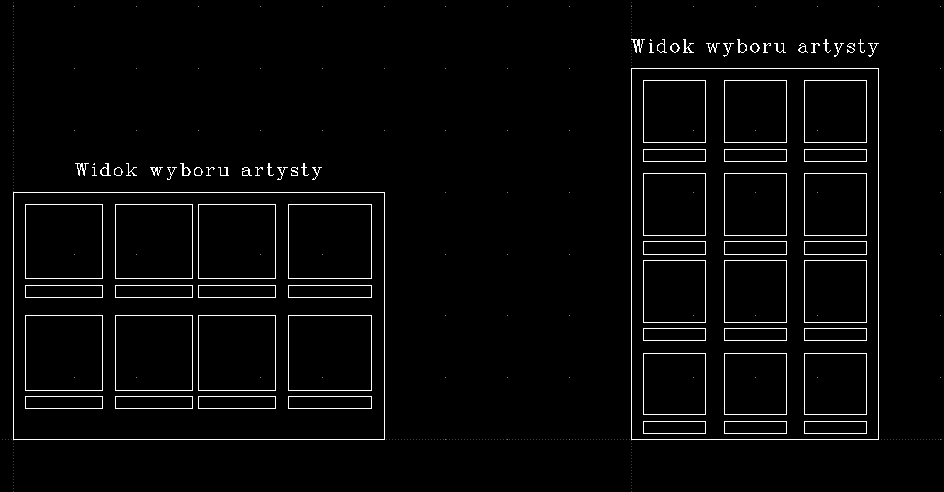
\includegraphics[width=1\textwidth]{images/mockup_artysta.png}
	\caption{\centering{Mockup widoku biblioteki - listing wykonawców}}
\end{figure}

Widok wykonawców będzie ekranem startowym aplikacji. "Kafelki" będa zdjęciami wykonawców. Klikanie na jeden z nich przejdzie do widoku albumów danego wykonawcy

\begin{figure}[H]
	\centering
	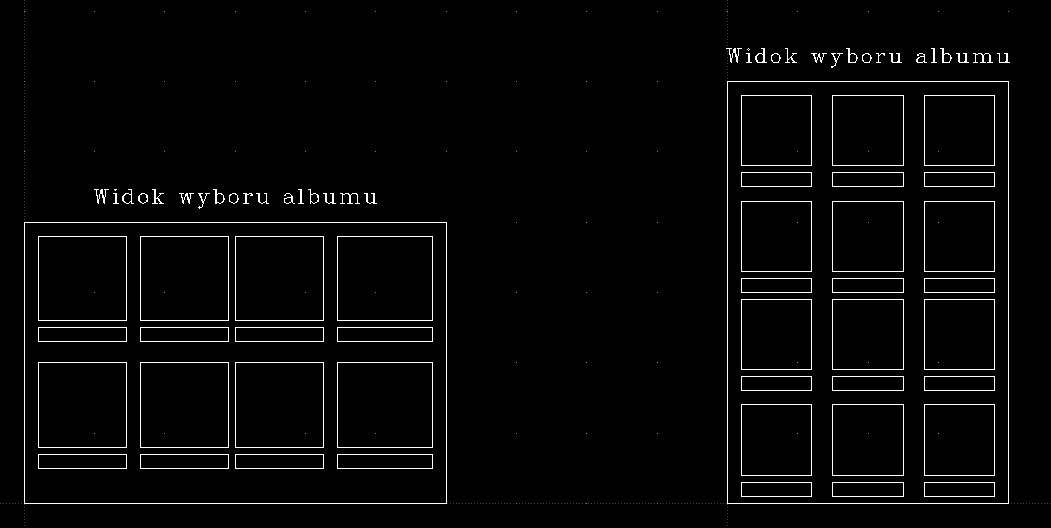
\includegraphics[width=1\textwidth]{images/mockup_albumy.png}
	\caption{\centering{Mockup widoku albumów danego wykonawcy}}
\end{figure}

Widok albumów jest identyczny jak widok wykonawców. Jedyna różnica polega tym, że zdjęcia na kafelkach będą zdjęciami albumów.

\begin{figure}[H]
	\centering
	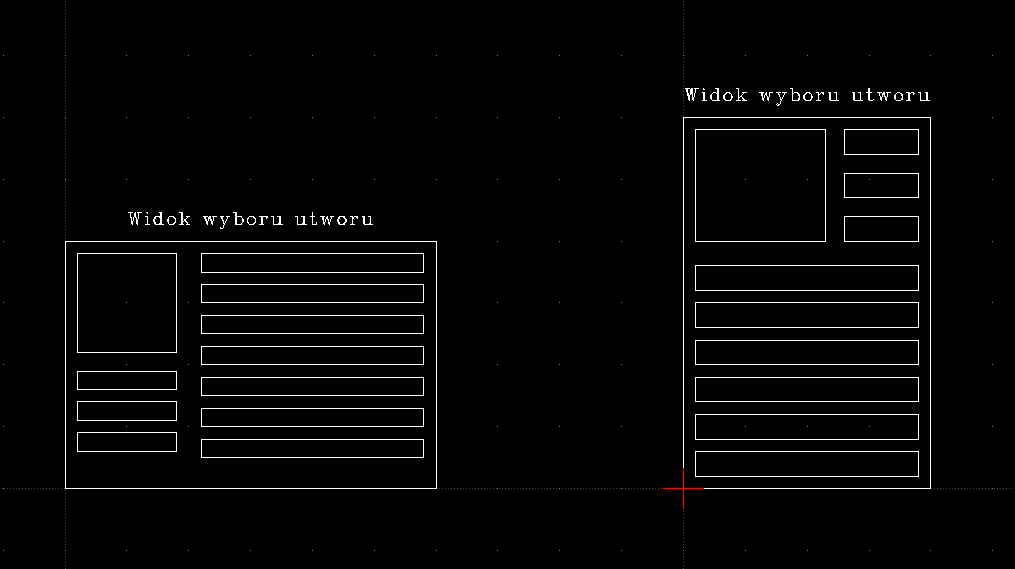
\includegraphics[width=1\textwidth]{images/mockup_utwory.png}
	\caption{\centering{Mockup widoku wyboru utworu}}
\end{figure}

Po wejściu na jakiś album zaprezentowane zostaną zawarte w nim utwory. W lewym górnym jest zdjęcie danego albumu, a obok niego jest kilka informacji o albumie jak wykonawca, data, tytuł. Dłuższe paski to lista tytułów piosenek, które można kliknąć, aby daną piosenkę włączyć.

\begin{figure}[H]
	\centering
	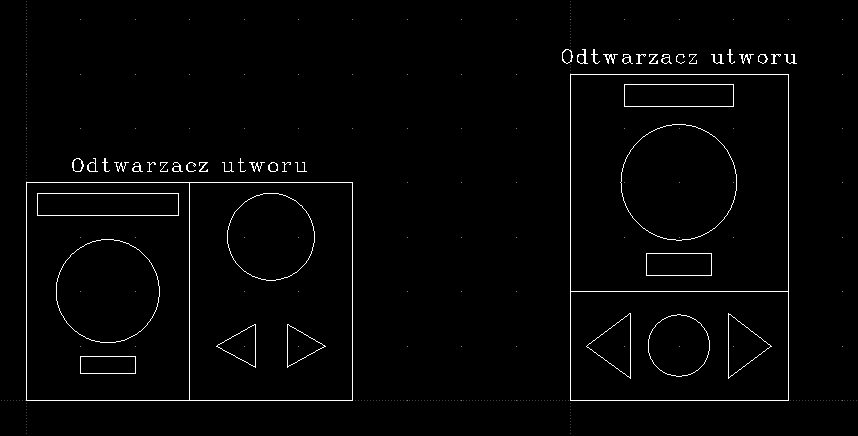
\includegraphics[width=1\textwidth]{images/mockup_odtwarzacz.png}
	\caption{\centering{Mockup odtwarzacza}}
\end{figure}

Odtwarzacz będzie działał następująco: duże koło będzie stylizowane na płytę, gdzie wypełniona ona będzie obrazem albumu. Płyta ta będzie się kręcić w czasie gdy gra piosenka. Kąt płyty (od 0\degree, do 360\degree) będzie określał jak duża część piosenki została odtworzona. Kąt ten będzie określony jeszcze niezdefiniowanym efektem graficznym. Prostokąty wokół płyty to tytuł piosenki, a na dole czas grania. Kółko i wokół niego trójkąty to przyciski odtwarzania - graj/pauza, następny, poprzedni. 

\begin{figure}[H]
	\centering
	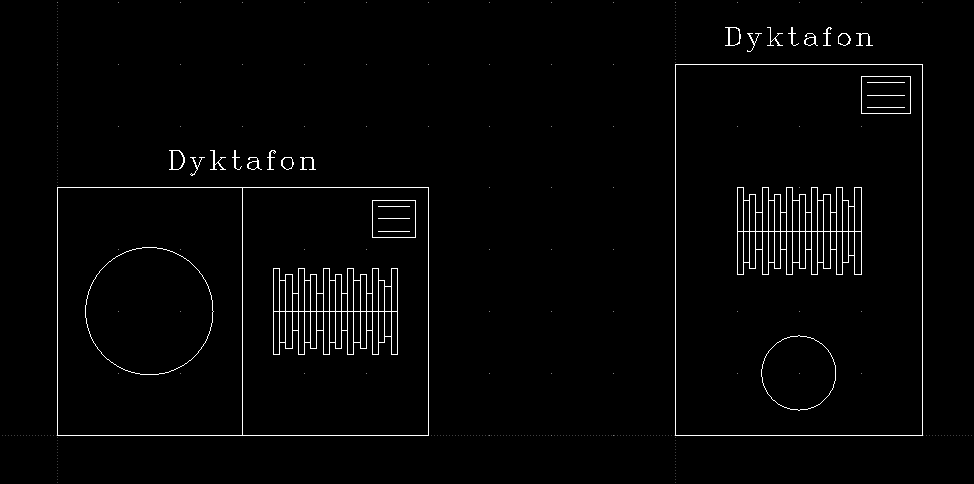
\includegraphics[width=1\textwidth]{images/mockup_dyktafon.png}
	\caption{\centering{Mockup dyktafonu}}
\end{figure}

Do dyktafonu będzie można się dostać przesuwając palcem w prawo na ekranie wykonawców. Dyktafon jest aktywowany wielkim okrągłym przyciskiem. Te kreski obok niego to wizualizacja dźwięku z mikrofonu. Menu w rogu będzie pozwalało na m.in. skonfigurowanie folderu zapisu nagrań.

\subsection{Zachowanie w niepożądanych sytuacjach}

Głównym wyjątkiem, na który może napotkać się aplikacja jest błąd odczytu albo plików, albo tagów z pliku. Kotlin, na szczęście, pozwala na łatwe sprawdzanie wartości null danych zmiennych operatorem '?'. W odpowiednich fragmentach kodu dotyczących ładowania plików, będzie sprawdzana poprawność danych i najprawdopodobniej pojawi się pop-up po stronie użytkownika, że wystąpił błąd, a po stronie dewelopera błąd zostanie logowany.

\subsection{Dalszy rozwój}

Jeżeli praca nad aplikacją będzie się odbywała w przyszłości, należy skupić uwagę na lepszym zarządzaniu biblioteką (auto tagowanie, pobieranie miniatur z internetu, itp.). Ponadto, należy szukać błędów, które nadal zostały w aplikacji.
